\chapter{Generative Adversarial Network (GAN)}
%\begin{refsection}

\begin{figure}[h!]
\centering
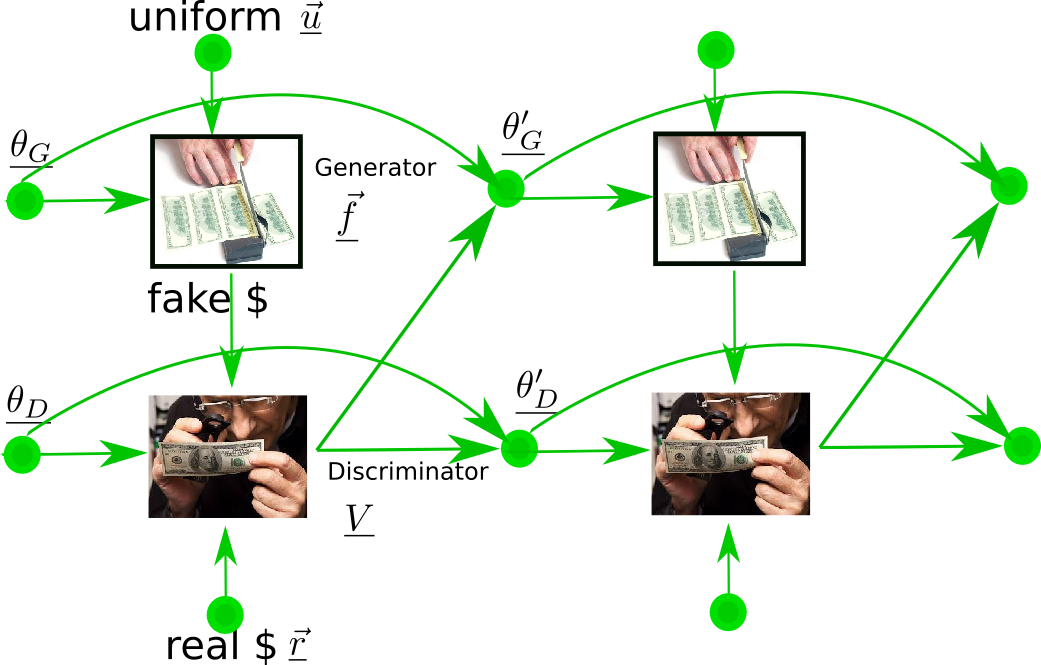
\includegraphics[width=6in]{gan/gan.png}
\caption{Generative Adversarial  Network (GAN)} 
\label{fig-gan}
\end{figure}

\begin{figure}[h!]
\centering
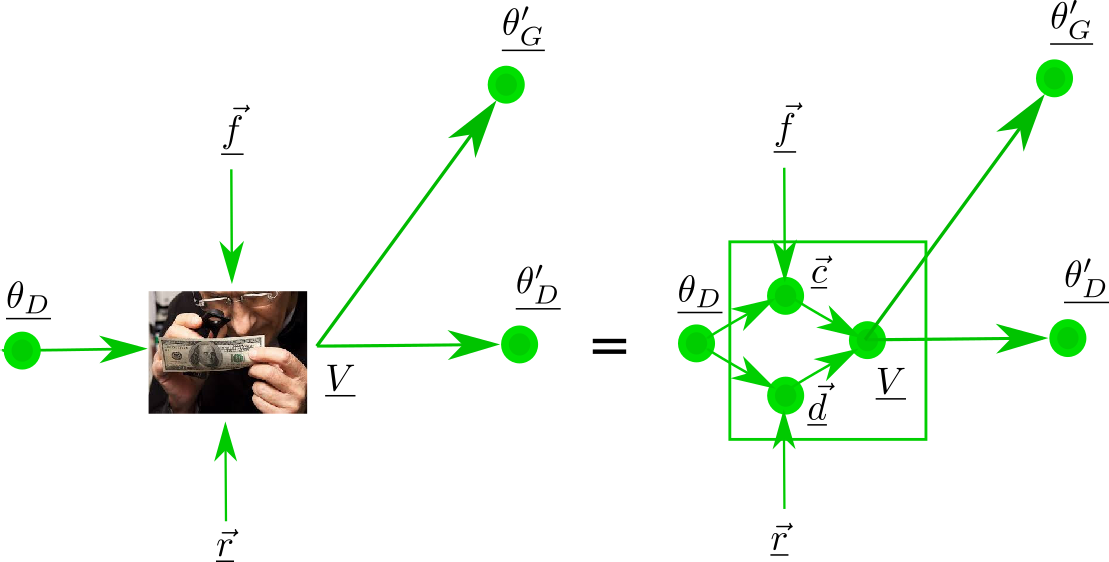
\includegraphics[width=6in]{gan/gan-detail.png}
\caption{Discriminator node $\ul{V}$ in Fig.\ref{fig-gan} can be
split into 3 nodes $\vec{\rvc}$, $\vec{\rvd}$ and $\ul{V}$.} 
\label{fig-gan-detail}
\end{figure}

Original GAN, 
Ref.\cite{gf2014}(2014). 

Generator $G$ (counterfeiter) generates samples $\vecf$ of fake money and submits them to Discriminator $D$ (Treasury agent). $D$ also gets samples $\vecr$ of real money. $D$ submits veredict $V\in [0,1]$. $G$ depends on parameter $\theta_G$ and $D$ on parameter $\theta_D$. Veredict $V$ and initial $\theta_G, \theta_D$ are used to get new parameters $\theta'_G, \theta'_D$.Process is repeated (Dynamical Bayesian Network) until saddle point in $V(\theta_G, \theta_D)$ is reached. $D$ makes $G$ better and vice versa.  Zero-sum game between $D$ and $G$.



Let $\cald$ be the domain of $D(\cdot, \theta_D)$. Assume that for any $x\in \cald$,

\beq
0\leq D(x,\theta_D)\leq 1
\;.
\eeq
For any $S\subset\cald$, define

\beq
\sum_{x\in S}D(x,\theta_D)=\lam(S,\theta_D)
\;.
\eeq


 In general, 
$G(\cdot,\theta_G)$ need not be real valued. 

Assume that for every $u\in S_\rvu$,
 $G(u,\theta_G)=f\in S_\rvf\subset \cald$. Define
\beq
\ol{D}(f,\theta_D)=1-D(f,\theta_D)
\;.
\eeq
Note that

\beq
0\leq\ol{D}(f,\theta_D)\leq 1
\;.
\eeq

Define:

\beq
V(\theta_G, \theta_D) =
\sum_{r}P(r)
\log D(r, \theta_D)
+ \sum_{u}P(u)\log
\ol{D}(G(u,\theta_G),\theta_D)
\;.	
\eeq

We want the first variation of $V(\theta_G, \theta_D)$ to vanish.




\beq
\delta V(\theta_G, \theta_D)=0
\;.
\eeq
This implies

\beq
 \partial_{\theta_G}V(\theta_G, \theta_D)=
 \partial_{\theta_D}V(\theta_G, \theta_D)=0
\;
\eeq
and

\beq
V_{opt}=\min_{\theta_G}\max_{\theta_D} V(\theta_G, \theta_D)
\;.
\eeq

Node transition  probability matrices
for Figs.\ref{fig-gan} and \ref{fig-gan-detail} 
are
given next in blue:

\beq\color{blue}
P(\theta_G)=\;{\rm given}
\eeq

\beq\color{blue}
P(\theta_D)=\;{\rm given}
\eeq


\beq\color{blue}
P(\vecu)=\prod_i P(u[i])  \;\;{\rm (usually \;uniform\; distribution)}
\eeq

\beq\color{blue}
P(\vecr)=\prod_i P(r[i])
\eeq


\beq\color{blue}
P(f[i]|\vecu, \theta_G)= \delta[f[i], G(u[i],\theta_G)]
\eeq

\beq\color{blue}
P(c[i]|\vecf, \theta_D) = \delta(c[i], \ol{D}(f[i], \theta_D))
\eeq

\beq\color{blue}
P(d[j]|\vecr, \theta_D)= \delta(d[j], D(r[j], \theta_D))
\eeq




\beq\color{blue}
P(V| \vecd,  \vecc)=
\delta(V, \frac{1}{N}\log \prod_{i,j}(c[i]d[j]))
\eeq
where $N=nsam(\vecr)nsam(\vecu)$.







Let $\eta_G, \eta_D> 0$. Maximize $V$ wrt $\theta_D$, and
minimize it wrt $\theta_G$.

\beq\color{blue}
P(\theta'_G|V,\theta_G )=
\delta(\theta'_G, \theta_G - \eta_G 
\partial_{\theta_G}V)
\eeq

\beq\color{blue}
P(\theta'_D|V,\theta_D )=
\delta(\theta'_D, \theta_D + \eta_D 
\partial_{\theta_D}V)
\eeq

\hrule
\begin{figure}[h!]
\centering
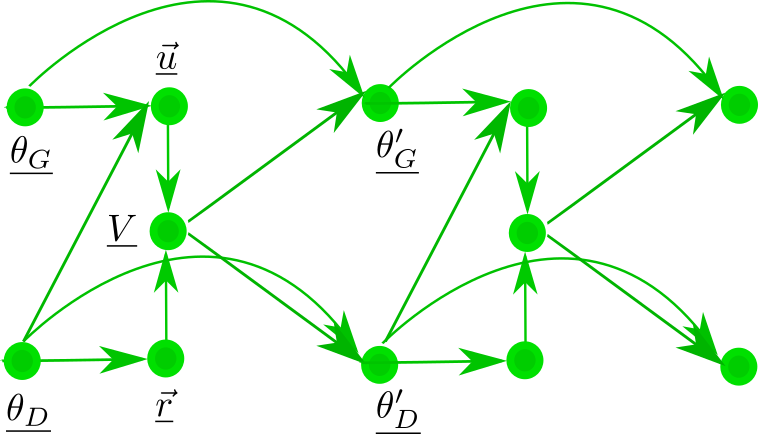
\includegraphics[width=2in]{gan/gan-emulate.png}
\caption{GAN, Constraining Bayesian Network}
\label{fig-gan-emulate} 
\end{figure}

Constraining B net given in Fig.\ref{fig-gan-emulate}. It adds 2 new nodes, namely $\ul{\vec{U}}$ and $\ul{\vec{R}}$, to  the bnet of Fig.\ref{fig-gan}. The purpose of these 2  barren (childrenless) nodes is to constrain certain functions to be probability distributions.

Node transition probabilities for the 2 new nodes given next in blue. 


\beq\color{blue}
P(U[i]|\theta_G)= 
\frac{\ol{D}(G(U[i],\theta_G),\theta_D))}
{\ol{\lam}(\theta_G, \theta_D)}
\eeq
where  $S_{\ul{U[i]}}=S_\rvu$ and $\ol{\lam}(\theta_G, \theta_D)=\sum_u\ol{D}(G(u, \theta_G), \theta_D))$.

\beq\color{blue}
P(R[i]|\theta_G, \theta_D)= \frac{D(R[i], \theta_D)}{\lam(\theta_D)}
\eeq
where $S_{\ul{R[i]}}=S_\rvr$ and  $\lam(\theta_D)=\sum_r D(r, \theta_D)$.


\beq\color{blue}
P(V| \vecu,  \vecr)=
\delta(V, \frac{1}{N}\log \prod_{i,j}(
P(\ul{R[i]}=r[i]|\theta_G, \theta_D)P(\ul{U[i]}=u[j]|\theta_G)))
\eeq
where $N=nsam(\vecr)nsam(\vecu)$.


$\call=$ likelihood
\beqa
\call&=&
P(\vecr, \vecu| \theta_G, \theta_D)\\
&=&
\prod_{i,j}\left[
 \frac{D(r[i], \theta_D)}{\lam(\theta_D)}
\frac{\ol{D}(G(u[j],\theta_G),\theta_D))}
{\ol{\lam}(\theta_G, \theta_D)}
\right]
\eeqa

\beq
\log \call = N[V(\theta_G, \theta_D)
-\log \lam(\theta_D)-\log \ol{\lam}(\theta_G, \theta_D)]
\eeq



%\printbibliography[heading=subbibliography]
%\end{refsection}


 